\begin{figure}[t]
\centering
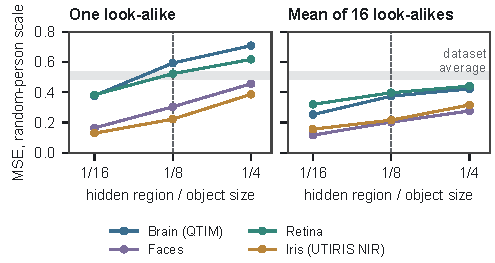
\includegraphics[width=\columnwidth]{fig/rq4_size.pdf}
\caption{\textbf{Nearest people come closer when the hidden region is small.}
\acs{MSE} on the random-person scale against the hidden-region size as a fraction of the object; lines average the sets of one modality (per image set: Supplementary Table~S13); gray band: dataset average; dashed line: the 1/8 used elsewhere.
The nearest person passes the dataset average in brain and retina from 1/8 on, while the mean of the 16 nearest people stays below it at every size.}
\label{fig:rq4}
\end{figure}
% Source: results/rq4_window_size.json; drawn by paper/cvpr2027/make_fig_rq4_size.py (values in fig/rq4_size_plotted.json).
